\mysection{Introduction}
\label{section:introduction}

Smart personal computing devices, such as phones, tablets, glasses, watches,
health monitors and other embedded devices have become an integral part of our
daily lives. We carry these devices as we go, and expect them to connect and
work with the environments that we visit.

While the increasing capability of smart devices and universal connectivity are
generally desirable trends, there are also environments where these trends may
be misused. In enterprise settings and federal institutions, for instance,
malicious personal devices can be used to exfiltrate sensitive information to
the outside world. In examination settings, smart devices may be used to
infiltrate unauthorized information~\cite{url:examcheating} or surreptiously
collude with peers~\cite{smartwatch:fc14} and cheat on the exam.  Even in less
stringent social settings, smart devices may be used to record pictures, videos
or conversations that could compromise privacy. We therefore need to regulate
the use of smart devices in such \textit{restricted spaces}.

Society currently relies on a number of \adhoc\ methods for policy enforcement
in restricted spaces. In the most stringent settings, such as in federal
institutions, employees may be required to place their personal devices in
Faraday cages and undergo physical checks before entering restricted spaces.
In corporate settings, employees often use separate devices for work and
personal computing needs. Personal devices are not permitted to connect to the
corporate network, and employees are implicitly, or by contract, forbidden from
storing corporate data on personal devices. In examination settings, proctors
ensure that students do not use unauthorized electronic equipment.  Other
examples in less formal settings include restaurants that prevent patrons from
wearing smart glasses~\cite{url:glassban}, or privacy-conscious individuals who
may request owners to refrain from using their devices.

We posit that such \adhoc\ methods alone will prove inadequate given our
increasing reliance on smart devices. For example, it is not possible to ask an
individual with prescription smart glasses (or other assistive health device)
to refrain from using the device in the restricted space. The right solution
would be to allow the glass to be used as a vision corrector, but regulate the
use of its peripherals, such as camera, microphone, or WiFi.  A general method
to regulate the use of smart devices in restricted spaces would benefit both
the \textit{hosts} who own or control the restricted space and \textit{guests}
who use smart devices.  Hosts will have greater assurance that smart devices
used in their spaces conform to their usage policies. On the other hand, guests
can benefit from and be more open about their use of smart devices in the
host's restricted space.\footnote{We only consider overt use of guest devices.
Covert use must still be addressed using other methods, such as physical
checks.}

Prior work on this problem
(\eg~\cite{asm:sec14,flaskdroid:sec13,conxsense:asiaccs14,worlddriven:ccs14,blindspot:2009,markit:upside14})
has typically assumed that guest devices are benign. The guest device is
outfitted with a security-enhanced software stack that is designed to accept
and enforce policies supplied by restricted space hosts. A host must trust the
software running on a guest device to correctly enforce its policies, and
generally has no means to obtain guarantees that a guest device is
policy-compliant. Clearly, a malicious guest device with a suitably-modified
software stack can easily bypass policy enforcement.

In this paper, we make two key advances. First, we leverage \textit{trusted
hardware} (the ARM TrustZone~\cite{armtz}) on guest devices to offer provable
security guarantees. In particular, a guest device can use the ARM TrustZone to
produce \textit{verification tokens}, which are unforgeable cryptographic
entities that establish to a host that the guest is policy-compliant.
Malicious guest devices, which may have violated the host's policies in the
restricted space, will not be able to provide such a proof, and can therefore
be apprehended by the host. Devices that use the ARM TrustZone are now
commercially available and widely deployed~\cite{knox:ccs14}, and our approach
applies to these devices.

\begin{figure*}[t!]
\begin{center}
\begin{tabular}{cc}
\begin{minipage}{0.47\textwidth}
\centering
\begin{tabular}{|c|}
\hline
\indent\vspace{-0.2cm}\\
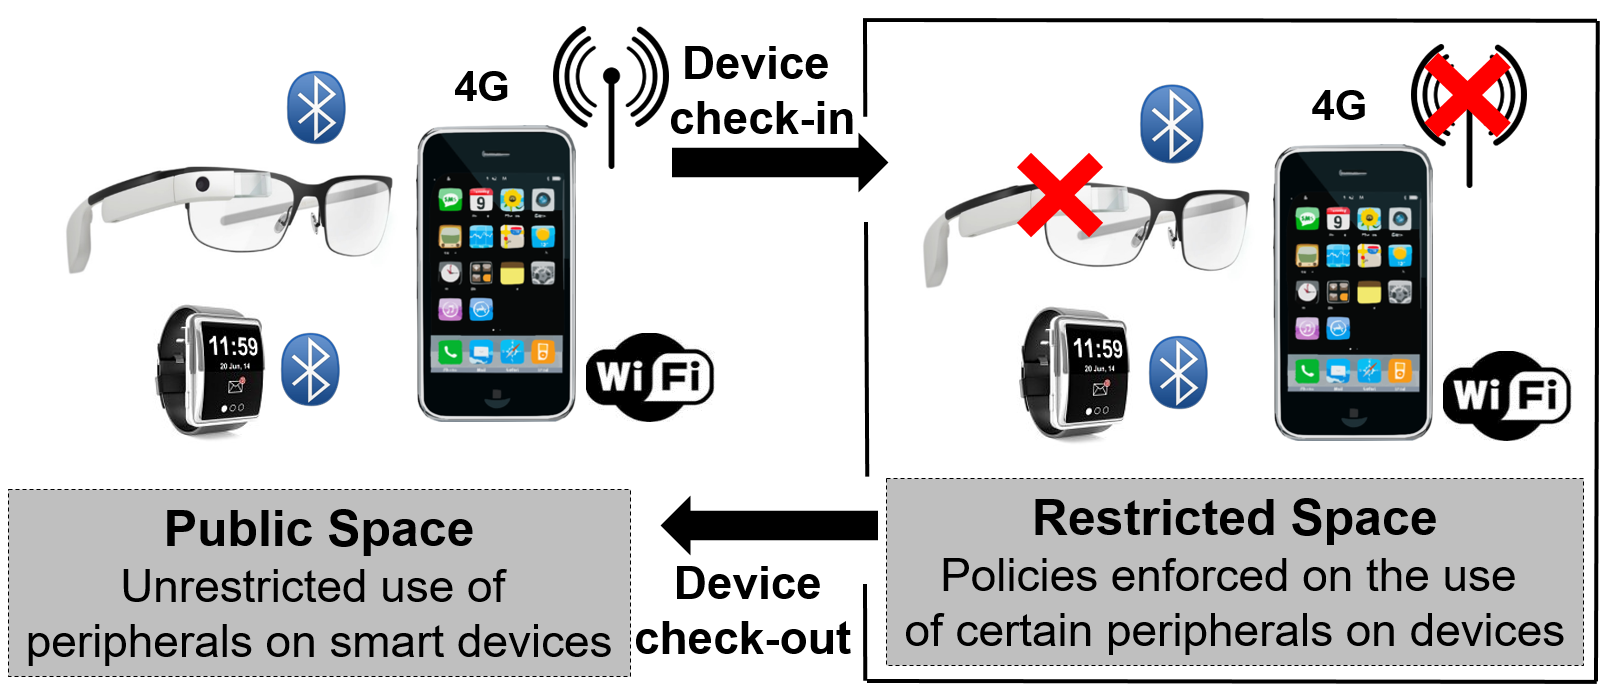
\includegraphics[keepaspectratio=true,width=0.95\textwidth]{figures/restricted-space.png}\\
\multicolumn{1}{|p{0.98\textwidth}|}
{\small Guests ``check-in'' devices when entering restricted spaces. During
check-in, hosts inspect, analyze and modify the configurations of these devices
in accordance with their usage policies. In this example, the host restricts
the use of the camera on the smart glass, and the 4G data interface on the
smart phone. However, the glass and watch can continue to use Bluetooth
pairing, while the phone can connect to the host's access points using WiFi.
When guests leave the restricted space, they ``check-out'' their devices,
restoring them to their original configurations.}\\
\hline
\end{tabular}
\end{minipage} &
\begin{minipage}{0.47\textwidth}
\centering
\begin{tabular}{|c|}
\hline
\indent\vspace{-0.2cm}\\
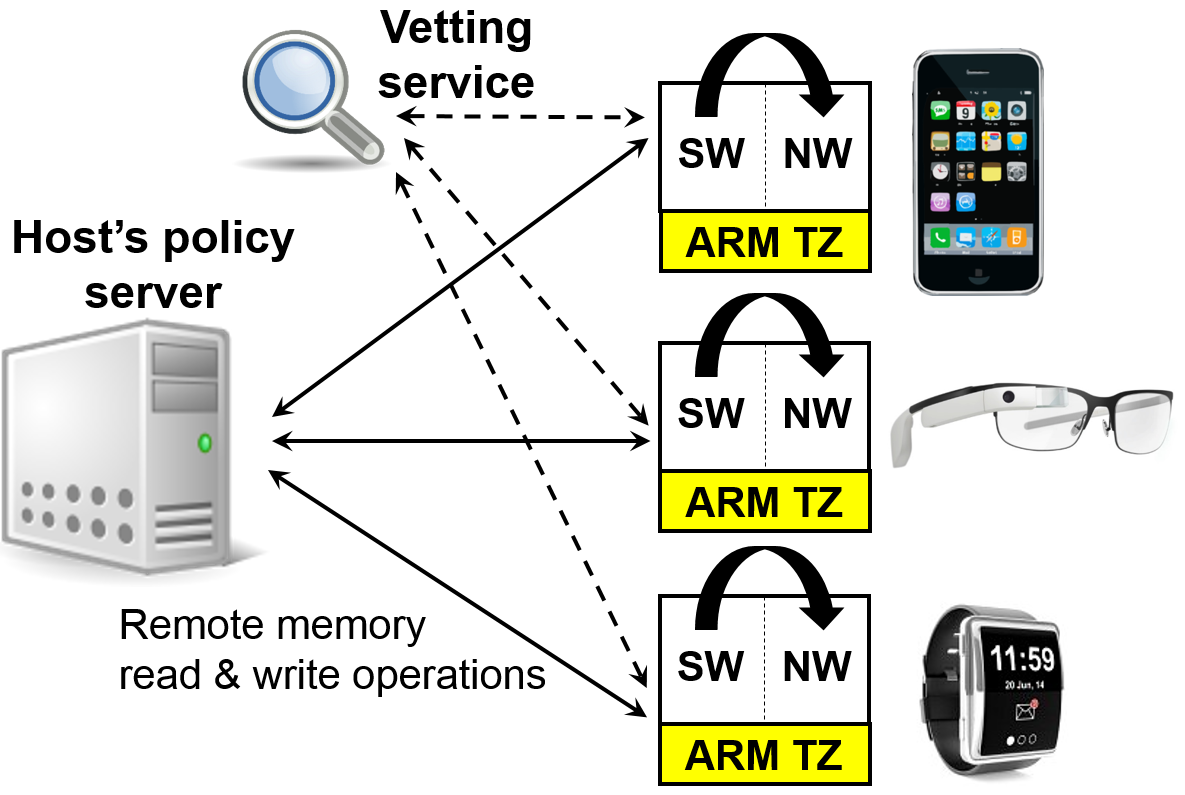
\includegraphics[keepaspectratio=true,width=0.90\textwidth]{figures/host-guest.png}\\
\multicolumn{1}{|p{0.98\textwidth}|}
{\small Guest devices are equipped with ARM TrustZone and execute components of
the policy enforcement mechanism in the secure world (SW). The details of this
mechanism appear in \sectref{section:mechanism}.  At check-in, the host's
policy server leverages the secure world to remotely inspect and modify normal
world (NW) memory.}\\
\hline
\end{tabular}
\end{minipage}
\end{tabular}
\end{center}
\indent\vspace{-0.5cm}
\mycaption{An overview of the entities of our restricted space model and the
setup of guest devices.}
{\label{figure:restrictedspaces}}
\end{figure*}

Second, we use host-initiated \textit{remote memory operations} as the core
method to regulate guest devices. In this approach, a host decides usage
policies that govern how guest devices must be regulated within the restricted
space. For example, the host may require a guest device to be free of certain
forms of malicious software, or that certain peripherals on the guest device
(\eg~camera, WiFi or 3G/4G) be disabled in the restricted space. The host
communicates these policies to the guest device, where a trusted
policy-enforcement mechanism applies these policies by reading or modifying
device memory. We show that the use of remote memory reads and writes
considerably simplifies the design and implementation of the policy-enforcement
mechanism, while still offering hosts fine-grained control over guest devices.
Remote memory operations also give hosts that use our approach the unique
ability to scan guest devices for kernel-level malware. Combined with the ARM
TrustZone, which helps bootstrap trust in the guest's policy-enforcement code,
our approach offers hosts an end-to-end guarantee that guest devices are
policy-compliant.

The two advances above benefit hosts, but guests may be uncomfortable with the
possibility of hosts accessing and modifying raw memory on their devices. We
therefore introduce a \textit{vetting service}, trusted and configurable by
guests, that allows them to check the safety of the host's memory operations
before performing them on the devices. The vetting service therefore
ameliorates guests' privacy concerns and restricts the extent to which hosts
can control their devices.

We built and evaluated a prototype to show the benefits of our approach. We
show that a small policy-enforcing code base running on guest devices offers
hosts fine-grained policy-based control over the devices. We also show that
with a few simple sanity checks, the vetting service allows guests to ensure
the safety of the host's remote memory operations.
